\section{Costruzione di un portfolio}

Per costruzione di un portfolio intendiamo distribuire la quota di investimento su certi asset (che siano stock, opzioni, bonds o qualsiasi altro strumento finanziario), l'obiettivo primario rimane nel bilanciare il rischio ed i potenziali profitti.

Il principio fondamentale utilizzato per la allocazione degli asset nel portfolio che stiamo creando di chiama \textbf{Modern Portfolio Theory} (\textbf{MPT} o analisi con media-varianza), MPT è stata creata
per aiutare gli investitori nella costruzione di un portfolio che massimizza i rendimenti per un livello di rischio specificato.

MPT è legato al concetto di \emph{diversificazione}, ciò significa che possedere diversi tipi di asset riduce il rischio, in quanto la perdita di rendimento di una particolare security ha meno impatto
sulla performance di portfolio. In principio minore è la correlazione tra gli asset nel portfolio, meglio è per la diversificazione.

\subsection{Costruzione del portfolio ottimale}

\subsubsection{Costruzione tramite simulazione di Monte Carlo}

Utilizziamo il metodo Monte Carlo per ottenere un set di portafogli ottimali (nella frontiera di efficienza), cioè:
\begin{itemize}
    \item Con il rendimento più alto dato un livello di rischio
    \item Con il più basso livello di rischio dato un livello di rendimento aspettato
\end{itemize}

\textbf{Utilizzando solo dati storici}

Utilizzando i dati storici (108 mesi) dei sei titoli relativi a questo progetto, eseguendo le simulazioni otteniamo come risultato il grafico a figura \ref{fig:pf_monte_carlo_1}.

\begin{figure}[ht]
    \centering
    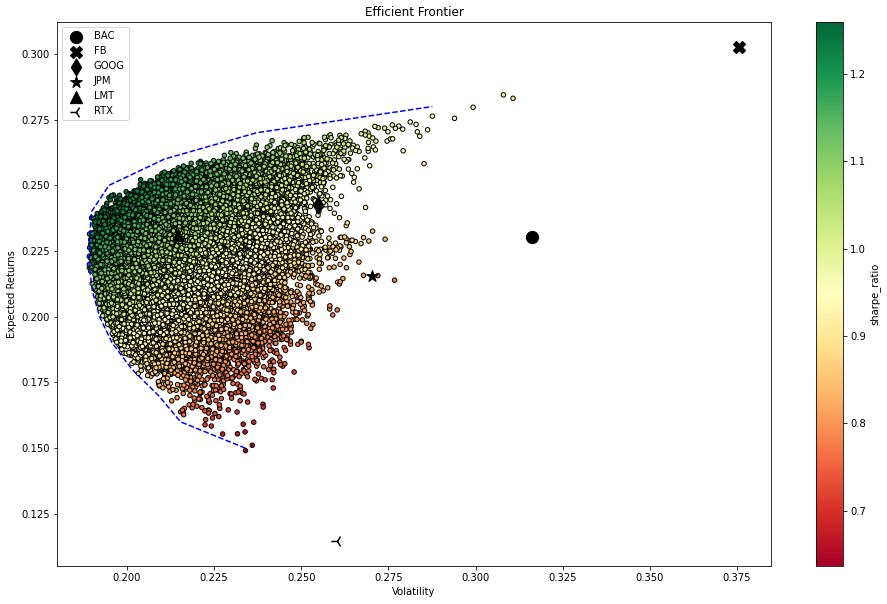
\includegraphics[width=1\textwidth]{portfolio_monte_carlo_1.png}
    \caption{Grafico con tutti i portafogli generati da Monte Carlo}
    \label{fig:pf_monte_carlo_1}
\end{figure}

\pagebreak

Dalle simulazioni eseguite identifichiamo vai portafogli che sono localizzati nella frontiera di efficienza, a figura \ref{fig:pf_monte_carlo_2} possiamo osservare
lo stesso grafico ma con evidenziati due portafogli sub-ottimali, uno con il rendimento più alto tra tutti e l'altro con la varianza più bassa.

\begin{figure}[ht]
    \centering
    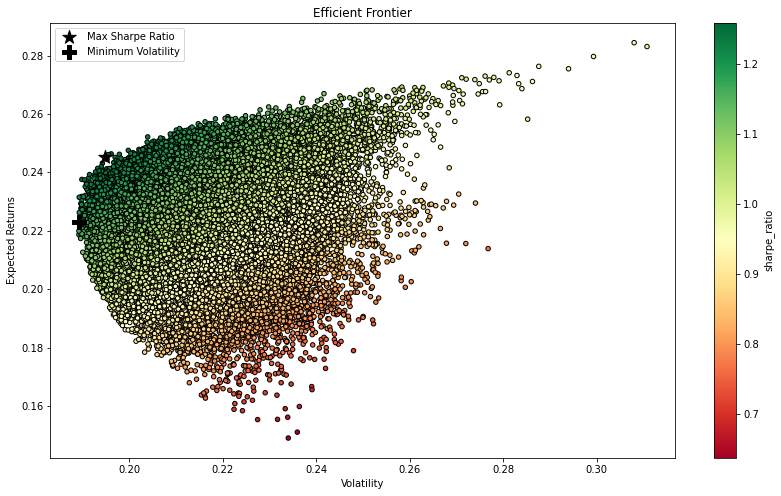
\includegraphics[width=1\textwidth]{portfolio_monte_carlo_2.png}
    \caption{Grafico con evidenza dei due portafogli sub-ottimali}
    \label{fig:pf_monte_carlo_2}
\end{figure}

La composizione del portafoglio sub-ottimale con il rendimento più alto la è la seguente (figura \ref{fig:pf_optimal_rd}).

\begin{figure}[ht]
    \centering
    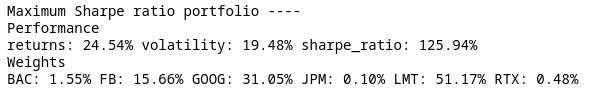
\includegraphics[width=.8\textwidth]{portfolio_optimal_rd.png}
    \caption{Composizione con pesi del portafoglio sub-ottimale con rendimento più alto}
    \label{fig:pf_optimal_rd}
\end{figure}

\textbf{Utilizzando i dati di previsione}

Applichiamo le simulazioni di Monte Carlo ai dati di previsione identificati nel capitolo 3 (su un periodo di 108 mesi).

La ripartizione della origine dei dati è la seguente:
\begin{itemize}
    \item Primi 80 mesi: Dati storici
    \item Dal mese 81 a 108: Dati di predizione
\end{itemize}